\chapter{Разработка и реализация процедур T-SQL}
\section{Разработка и реализация хранимых процедур}

Хранимые процедуры — это процедуры, которые находятся в базе данных и
инкапсулируют код. 


\subsection{Основные сведения о хранимых процедурах }


В действительности почти все инструкции
T-SQL могут быть включены в хранимую процедуру. Однако надо учесть следующее: 

\begin{itemize}
	\item нельзя использовать команду USE <database name>; 
	\item нельзя использовать инструкцию CREATE с любым из следующих типов объектов: AGGREGATE, RULE, DEFAULT, CREATE, FUNCTION, TRIGGER, PROCEDURE или VIEW; 
	\item можно создать, изменить и удалить таблицу и индекс с помощью инструкций
	CREATE, ALTER и DROP. 
\end{itemize}

\subsection{Параметры хранимой процедуры}


\begin{lstlisting}[label=lst:funcReturn, language=sql]
	CREATE PROC Sales.GetCustomerOrders
		@custid AS INT,
		@orderdatefrom AS DATETIME = '19000101',
		@orderdateto AS DATETIME = '99991231',
		@numrows AS INT = 0 OUTPUT
   AS
   BEGIN
		SET NOCOUNT ON;
		SELECT orderid, custid, shipperid, orderdate, requireddate, shippeddate
		FROM [Sales].[Orders]
		WHERE custid = @custid
		AND orderdate >= @orderdatefrom
		AND orderdate < @orderdateto;
		SET @numrows = @@ROWCOUNT;
   		RETURN;
	END 
\end{lstlisting}

\begin{itemize}
	\item Параметры могут быть обязательными или необязательными. При отсутствии инициализации по умолчанию параметр является обязательным. В предыдущем коде @custid — это обязательный параметр. 
	\item Ключевое слово OUTPUT определяет специальный параметр, который возвращает
	значения вызывающей стороне. Выходные параметры всегда являются необязательными параметрами. 
	\item Команда AS обязательно должна стоять после списка параметров. 
\end{itemize}

\subsection{Блок BEGIN/END}
Можно заключить код в хранимой процедуре в блок BEGIN/END. Хотя это не является обязательным требованием, использование блока BEGIN/END помогает сделать код
более понятным. 

\subsection{Инструкция SET NOCOUNT ON}
Можно встроить инструкцию NOCOUNT со значением ON внутрь хранимой процедуры,
чтобы запретить вывод сообщений, подобный (3 row(s) affected), при каждом
выполнении процедуры. 

\begin{figure}[h!]
	\begin{center}
		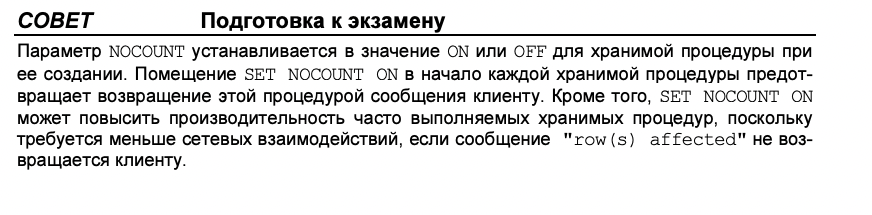
\includegraphics[width=0.9\textwidth]{img/advice32.png}
	\end{center}
	\captionsetup{justification=centering}
\end{figure}

\subsection{Команда RETURN и коды возврата}

В одной процедуре можно использовать более одной команды RETURN. Эта команда
останавливает выполнение процедуры и возвращает управление обратно вызывающей стороне.

При успешном выполнении статус равен 0, при наличии
ошибки статус равен отрицательному числу. Но не следует полагаться на номера
ошибок, т. к. они не надежны. Вместо этого следует использовать номера ошибок
SQL Server, возвращаемые функцией @@ERROR или функцией ERROR\_NUMBER(), вызываемой в блоке CATCH. 


\begin{figure}[h!]
	\begin{center}
		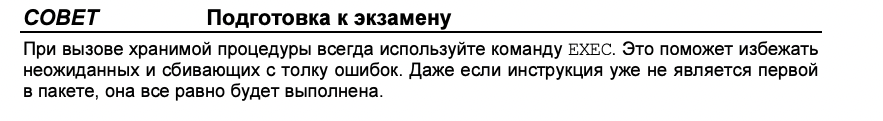
\includegraphics[width=0.9\textwidth]{img/advice33.png}
	\end{center}
	\captionsetup{justification=centering}
\end{figure}


\begin{figure}[h!]
	\begin{center}
		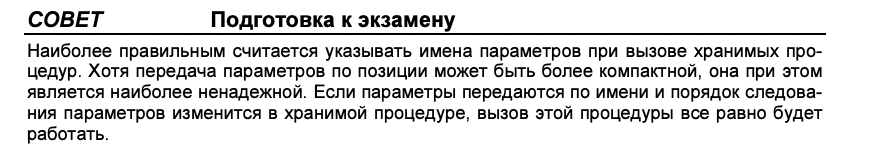
\includegraphics[width=0.9\textwidth]{img/advice36.png}
	\end{center}
	\captionsetup{justification=centering}
\end{figure}


\subsection{Логика ветвления}

К инструкциям управления потоком выполнения относятся следующие: 

\begin{itemize}
	\item IF/ELSE; 
	\item WHILE (c BREAK и CONTINUE); 
	\item WAITFOR; 
	\item GOTO; 
	\item RETURN (обычно внутри процедур T-SQL). 
\end{itemize}


\subsection{Конструкция IF/ELSE}

\begin{lstlisting}[label=lst:funcReturn, language=sql]
	DECLARE @var1 AS INT, @var2 AS INT;
	SET @var1 = 1;
	SET @var2 = 2;
	IF @var1 = @var2
	 PRINT 'The variables are equal';
	ELSE
	 PRINT '@var1 equals @var2';
	GO 
\end{lstlisting}


Если инструкции IF или ELSE используются без блока BEGIN/END, каждая из них обрабатывает только одну инструкцию.

\subsection{Конструкция WHILE}


\begin{lstlisting}[label=lst:funcReturn, language=sql]
	SET NOCOUNT ON;
	DECLARE @count AS INT = 1;
	WHILE @count <= 10
	 BEGIN
	 PRINT CAST(@count AS @count);
	 SET @count += 1;
	 END; 
\end{lstlisting}

\begin{figure}[h!]
	\begin{center}
		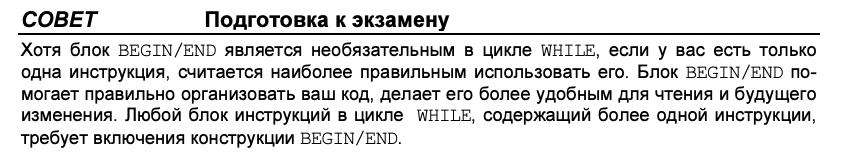
\includegraphics[width=0.9\textwidth]{img/advice37.png}
	\end{center}
	\captionsetup{justification=centering}
\end{figure}

Важно отметить, что когда условие WHILE тестирует элементы, которые могут содержать дубликаты, оно захватывает только их общее значение, пропуская все остальные.


\subsection{Команда WAITFOR}

\begin{lstlisting}[label=lst:funcReturn, language=sql]
	DECLARE @categoryname AS NVARCHAR(15);
	SET @categoryname = (SELECT MIN(categoryname) FROM Production.Categories);
	WHILE @categoryname IS NOT NULL
	BEGIN
	 PRINT @categoryname;
	 SET @categoryname = (SELECT MIN(categoryname) FROM Production.Categories
	 WHERE categoryname > @categoryname);
	END;
	GO
\end{lstlisting}

\subsection{Команда WAITFOR}

Команда WAITFOR имеет
три варианта: WAITFOR DELAY, WAITFOR TIME и WAITFOR RECEIVE (WAITFOR RECEIVE используется только с компонентом Service Broker). 
Опция WAITFOR DELAY вызывает задержку выполнения на указанный период времени. Например, следующий код останавливает выполнение кода на 20 секунд. 

\begin{lstlisting}[label=lst:funcReturn, language=sql]
	WAITFOR DELAY '00:00:20';
\end{lstlisting}

Опция WAITFOR TIME приостанавливает выполнение до указанного времени. Например, следующий код ждет до 23:45. 

\begin{lstlisting}[label=lst:funcReturn, language=sql]
	WAITFOR TIME '23:46:00';
\end{lstlisting}

\subsection{Вызов других хранимых процедур}
Если временная таблица создается в одной хранимой процедуре — например,
назовем ее Proc1, — эта временная таблица видна всем другим хранимым процедурам, вызываемым из Proc1. Но эта временная таблица не видна процедурам,
вызывающим Proc1. Переменные, объявленные в Proc1, и параметры процедуры Proc1 не видны никаким процедурам, вызываемым процедурой Proc1. 

\begin{figure}[h!]
	\begin{center}
		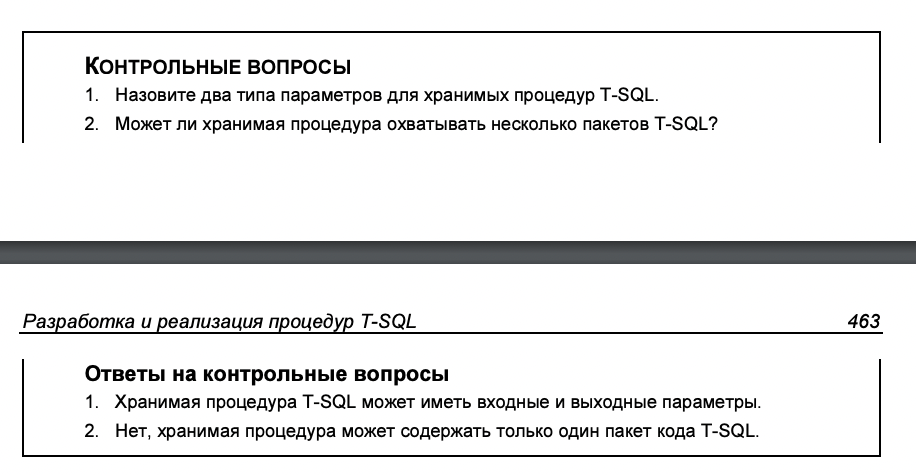
\includegraphics[width=0.9\textwidth]{img/control38.png}
	\end{center}
	\captionsetup{justification=centering}
\end{figure}




\subsection*{Резюме занятия}
\begin{itemize}
	\item Хранимые процедуры T-SQL — это модули кода T-SQL, которые хранятся в базе данных и могут быть выполнены с помощью команды T-SQL EXECUTE. 
	\item Хранимые процедуры можно использовать для инкапсуляции кода на стороне
	сервера, что снижает нагрузку на сеть со стороны приложений; для представления приложениям уровня доступа к данным; для выполнения административных
	задач и техобслуживания. 
	\item Хранимые процедуры можно определить с помощью параметров. Входные параметры отправляются хранимой процедуре для внутреннего использования процедуры. Выходные параметры могут использоваться для возвращения информации вызывающей стороне. 
	\item Внутри хранимой процедуры параметры определяются с помощью такого же
	синтаксиса, что и переменные T-SQL, и на них можно ссылаться и манипулировать ими внутри процедуры точно так же, как это происходит с переменными. 
	\item Каждая хранимая процедура состоит только из одного пакета кода T-SQL. Хранимые процедуры могут вызывать другие хранимые процедуры. 
	\item Где бы ни выполнялась команда RETURN, выполнение хранимой процедуры
	заканчивается и управление возвращается вызывающей стороне. 
	\item Хранимые процедуры могут возвращать вызывающей стороне более одного
	результирующего набора. 
\end{itemize}

\subsection*{Закрепление материала}

\begin{figure}[h!]
	\begin{center}
		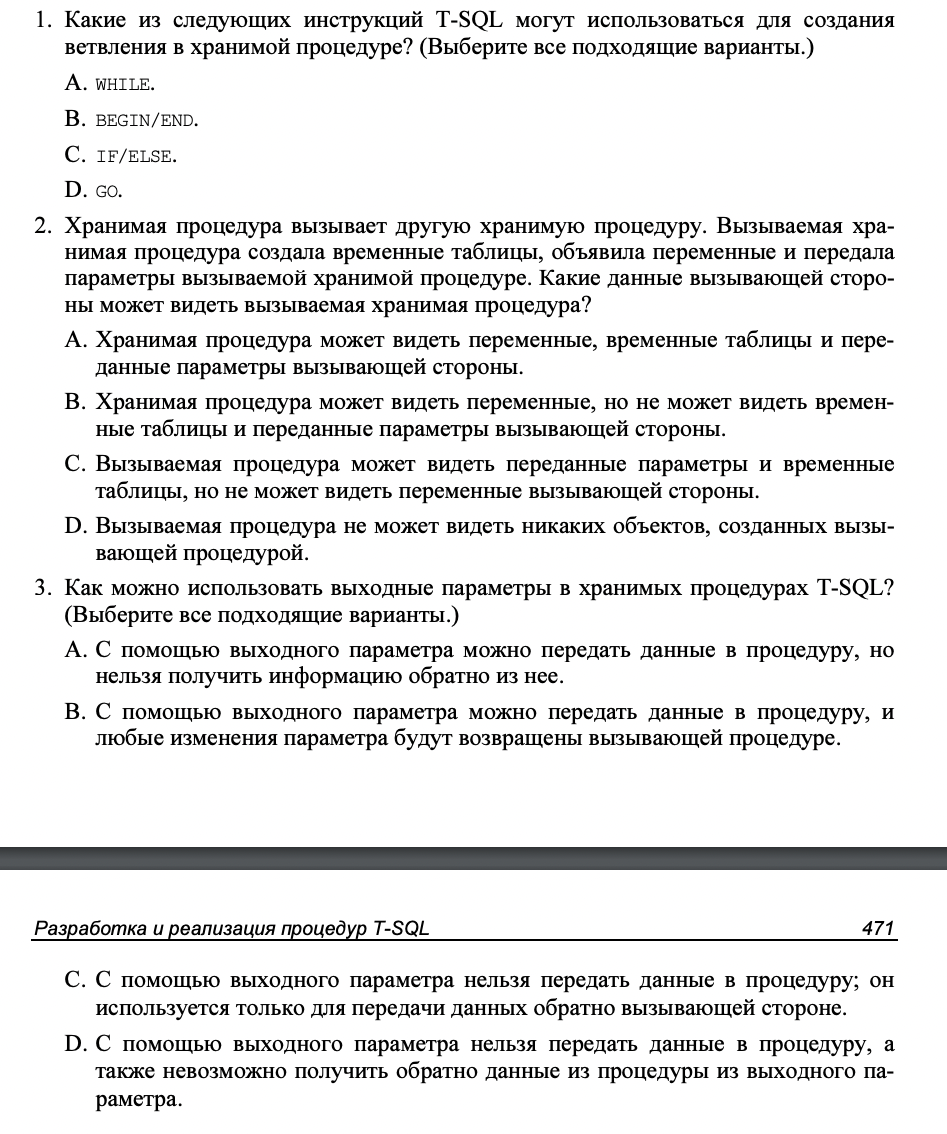
\includegraphics[width=0.7\textwidth]{img/zakrep30.png}
	\end{center}
	\captionsetup{justification=centering}
\end{figure}
\newpage

\subsection*{Ответы}

\begin{figure}[h!]
	\begin{center}
		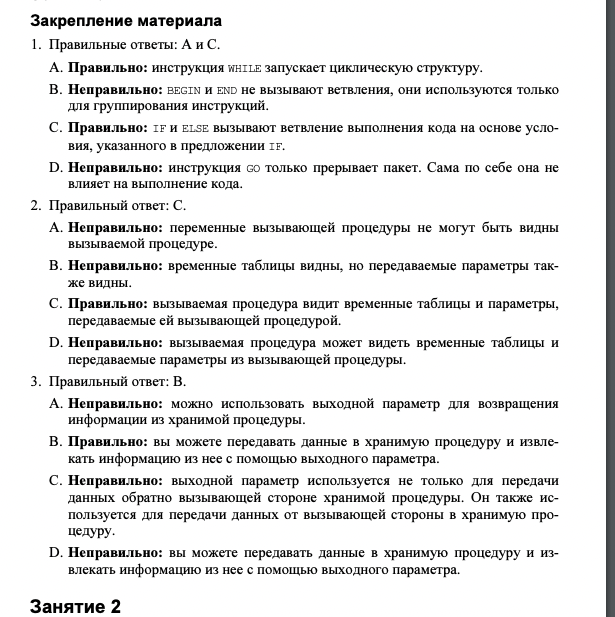
\includegraphics[width=0.9\textwidth]{img/ans30.png}
	\end{center}
	\captionsetup{justification=centering}
\end{figure}
\clearpage



\section{Реализация триггеров}

Триггер — это особый тип хранимой процедуры, связанный с выбранными
событиями языка обработки данных в таблице или представлении. Триггер
не может быть выполнен явно. Он срабатывает, когда запускает событие
DML, связанное с этим триггером, такое как инструкции INSERT, UPDATE или DELETE. 


\subsection{Триггеры DML}

Триггер DML — это пакет T-SQL, связанный с таблицей, которая предназначена для того, чтобы отвечать на определенное событие DML, такое как
инструкция INSERT, UPDATE или DELETE, или комбинацию этих событий.

\begin{itemize}
	\item AFTER — этот триггер срабатывает после того, как событие, с которым он связан,
	завершается, и может быть определен только для постоянных таблиц; 
	\item INSTEAD OF — этот триггер срабатывает вместо события, с которым он связан,
	и может быть определен в постоянных таблицах и представлениях. 
\end{itemize}

Оба типа триггеров DML выполняются как часть транзакции, связанной с инструкцией INSERT, UPDATE или DELETE. Триггер рассматривается как часть транзакции, которая включает событие, вызывающее срабатывание триггера. 

\subsection{Триггеры AFTER}

\begin{lstlisting}[label=lst:funcReturn, language=sql]
	CREATE TRIGGER Sales.tr_SalesOrderDetailsDML
	ON Sales.OrderDetails
	FOR DELETE, INSERT, UPDATE
	AS
	BEGIN
	 SET NOCOUNT ON
	END 
\end{lstlisting}

Прежде всего, убедитесь в том, что это триггер AFTER. В определении триггера типом по умолчанию является AFTER, если указан элемент FOR. Но элемент FOR может
быть заменен либо AFTER, либо INSTEAD OF для определения типа триггера. 

\subsection{Оптимизация триггера}

\begin{figure}[h!]
	\begin{center}
		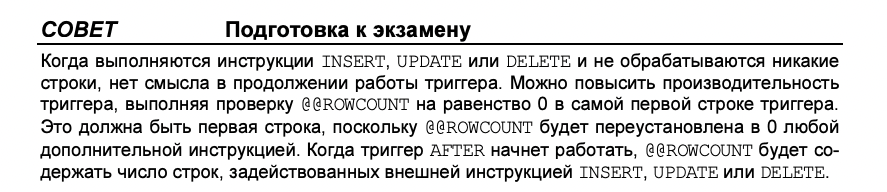
\includegraphics[width=0.9\textwidth]{img/advice38.png}
	\end{center}
	\captionsetup{justification=centering}
\end{figure}

\begin{lstlisting}[label=lst:funcReturn, language=sql]
	CREATE TRIGGER Sales.tr_SalesOrderDetailsDML
	ON Sales.OrderDetails
	AFTER DELETE, INSERT, UPDATE
	AS
	BEGIN
	 IF @@ROWCOUNT = 0 RETURN;
	 SET NOCOUNT ON;
	 SELECT COUNT(*) AS InsertedCount FROM Inserted;
	 SELECT COUNT(*) AS DeletedCount FROM Deleted;
	END;
\end{lstlisting}


\begin{figure}[h!]
	\begin{center}
		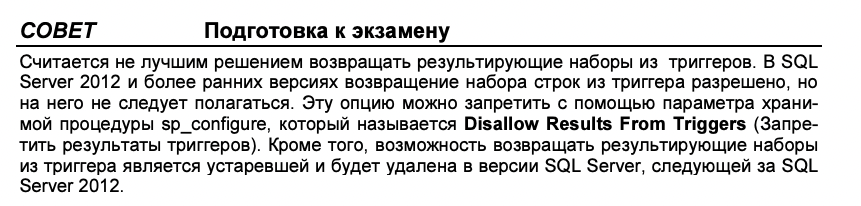
\includegraphics[width=0.9\textwidth]{img/advice39.png}
	\end{center}
	\captionsetup{justification=centering}
\end{figure}


\subsection{Триггеры INSTEAD OF}
Хотя триггеры INSTEAD OF могут создаваться как для таблиц, так и для представлений, обычно они используются с представлениями. Причина в том, что когда инструкция UPDATE отправляется к представлению, может быть обновлена только одна
таблица за один раз. Кроме того, в представлении могут быть агрегаты функций на
столбцах, не допускающие прямого обновления. Триггер INSTEAD OF может взять
инструкцию UPDATE применительно к представлению и, вместо ее выполнения, заменить ее двумя инструкциями UPDATE применительно к базовой таблице представления.


\begin{lstlisting}[label=lst:funcReturn, language=sql]
CREATE TRIGGER Production.tr_ProductionCategories_categoryname
ON Production.Categories
INSTEAD OF INSERT
AS
BEGIN
	SET NOCOUNT ON;
	IF EXISTS (SELECT COUNT(*)
		FROM Inserted AS I
		LEFT JOIN Production.Categories AS C
			ON I.categoryname = C.categoryname
		GROUP BY I.categoryname
		HAVING COUNT(*) > 0 )
		BEGIN
			THROW 50000, 'Duplicate category names not allowed', 0;
		END;
	ELSE
		INSERT Production.Categories (categoryname, description)
		SELECT categoryname, description FROM Inserted;
END; 
\end{lstlisting}


\subsection{Функции триггеров DML}

Для получения информации о том, что происходит в коде, можно использовать
в триггере две функции. 
\begin{itemize}
	\item UPDATE(). Эту функцию можно использовать, чтобы определить, имеет ли конкретный столбец ссылки от инструкций INSERT или UPDATE. Например, можно
	вставить в триггер следующий код: IF UPDATE(qty) PRINT 'Column qty affected';
	\item COLUMNS\_UPDATED(). Можно использовать эту функцию, если известен последовательный номер столбца в таблице. Вы должны будете использовать битовую операцию  И чтобы проверить, был ли столбец обновлен. 
\end{itemize}


\begin{figure}[h!]
	\begin{center}
		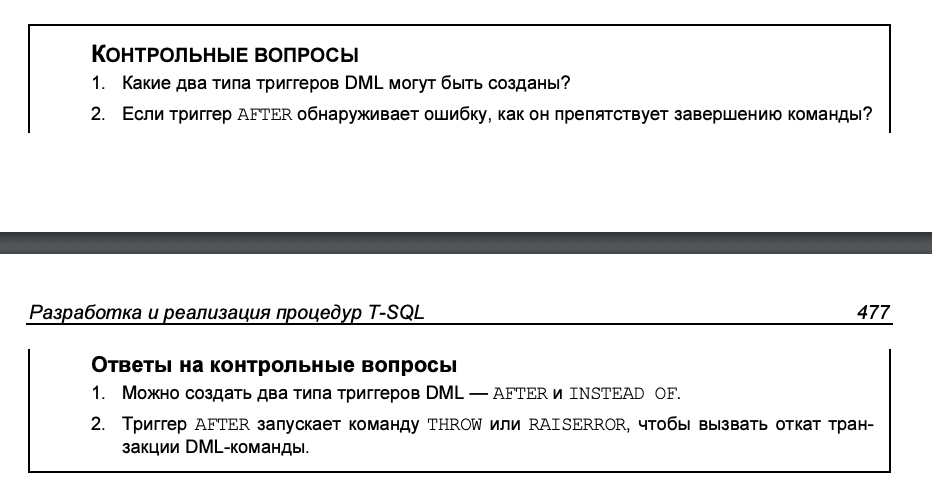
\includegraphics[width=0.9\textwidth]{img/control39.png}
	\end{center}
	\captionsetup{justification=centering}
\end{figure}

		
\subsection*{Резюме занятия}
\begin{itemize}
\item Триггер DML — это пакет кода T-SQL, подобный хранимой процедуре, который
связан с таблицей и иногда с представлением. Триггеры DML могут использоваться для аудита, реализации сложных правил целостности и т. п. 
\item Триггеры выполняются, когда происходит определенное событие DML, такое
как инструкция INSERT, UPDATE или DELETE. 
\item SQL Server поддерживает два типа триггеров DML: триггеры AFTER и триггеры
INSTEAD OF. Триггеры DML обоих типов выполняются как часть транзакции, связанной с инструкциями INSERT, UPDATE или DELETE. 
\item В коде T-SQL для обоих типов триггеров DML можно получить доступ к таблицам, называемым вставленными и удаленными таблицами. Эти таблицы содержат строки, модификация которых приводила к запуску триггера. 
\end{itemize}



\subsection*{Закрепление материала}

\begin{figure}[h!]
	\begin{center}
		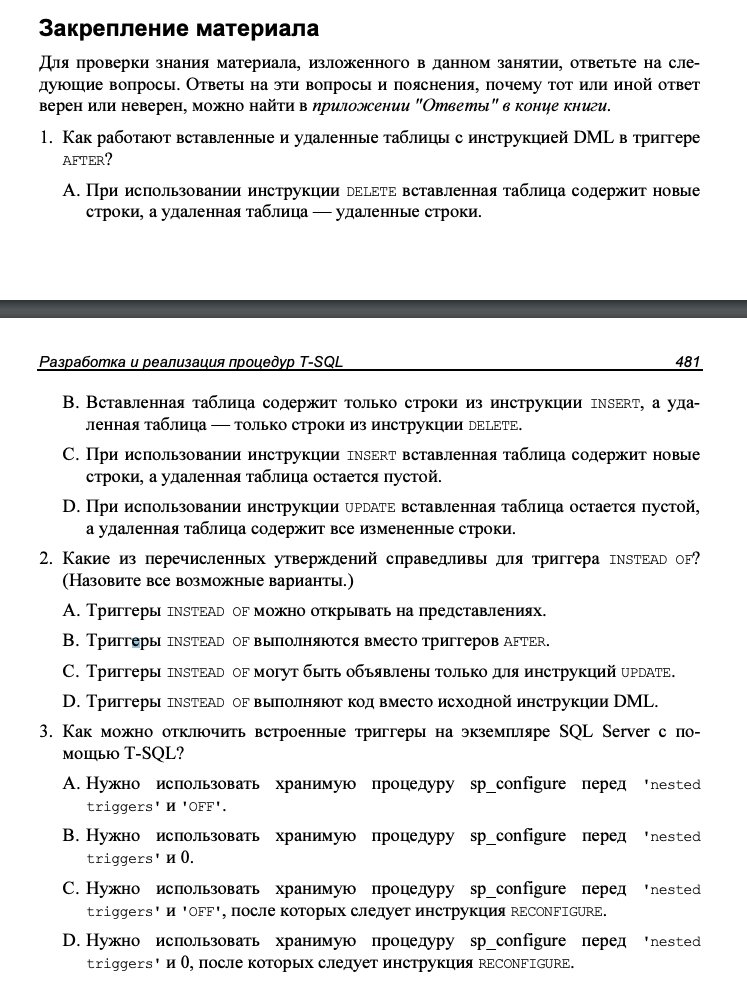
\includegraphics[width=0.9\textwidth]{img/zakrep31.png}
	\end{center}
	\captionsetup{justification=centering}
\end{figure}
\clearpage

\subsection*{Ответы}

\begin{figure}[h!]
	\begin{center}
		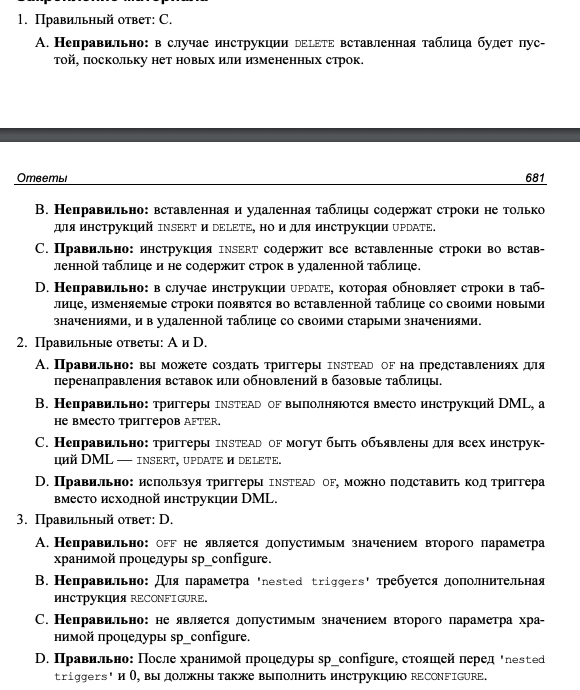
\includegraphics[width=0.9\textwidth]{img/ans31.png}
	\end{center}
	\captionsetup{justification=centering}
\end{figure}



\section{Основные сведения
об определяемых пользователем функциях}


В отличие от хранимых процедур, определяемые пользователем функции
встроены в инструкции T-SQL и выполняются как часть команды T-SQL. Определяемые пользователем функции не могут выполняться с помощью команды
EXECUTE. 

Определяемые пользователем функции имеют доступ к данным SQL Server, но не
могут выполнять DDL, т. е. они не могут создавать таблицы, а также модифицировать таблицы, индексы или любые другие объекты или изменять любые данные
в постоянных таблицах с помощью инструкций DML. 


\subsection{Скалярные определяемые пользователем функции}


\begin{lstlisting}[label=lst:funcReturn, language=sql]
	CREATE FUNCTION dbo.FunctionName
	( @param1 int,
	 @param2 int)
	RETURNS INT
	AS
	BEGIN
	 RETURN @param1 + @param2
	END 
\end{lstlisting}



\subsection{Встроенная пользовательская функция с табличным значением}

\begin{lstlisting}[label=lst:funcReturn, language=sql]
	CREATE FUNCTION dbo.FunctionName
	( @param1 int,
	 @param2 char(5) )
	RETURNS TABLE AS RETURN
	( SELECT @param1 AS c1,
	 @param2 AS c2 )
\end{lstlisting}



\subsection{Многооператорная пользовательская функция с табличным значением}

\begin{lstlisting}[label=lst:funcReturn, language=sql]
	CREATE FUNCTION dbo.FunctionName
	( @param1 int,
	 @param2 char(5) )
	RETURNS @returntable TABLE
	( c1 int,
	 c2 char(5) )
	AS
	BEGIN
	 INSERT @returntable
	 SELECT @param1, @param2
	 RETURN
	END;
\end{lstlisting}


\subsection{Ограничения для определяемых пользователем функций}

Определяемые пользователем функции не могут выполнять следующие действия: 
\begin{itemize}
	\item применять какие-либо изменения к схеме или данным в базе данных; 
	\item изменять состояние базы данных или экземпляра SQL Server; 
	\item создавать временные таблицы или иметь к ним доступ; 
	\item вызывать хранимые процедуры; 
	\item выполнять динамический SQL; 
	\item производить побочные эффекты. Например, функции RAND() и NEWID() используют информацию из предыдущего вызова. Использование предыдущей информации является "побочным эффектом", что недопустимо. 
	\item 
\end{itemize}


\begin{figure}[h!]
	\begin{center}
		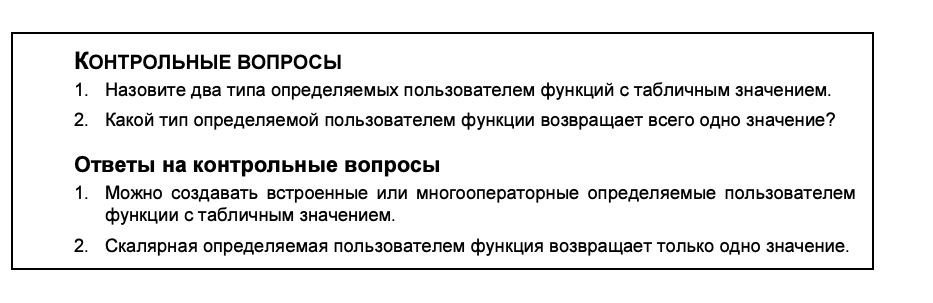
\includegraphics[width=0.9\textwidth]{img/control40.png}
	\end{center}
	\captionsetup{justification=centering}
\end{figure}


\subsection*{Резюме занятия}
\begin{itemize}
	\item Определяемые пользователем функции инкапсулируют повторно используемый код T-SQL и возвращают вызывающей стороне скалярное значение или
	таблицу. 
	\item Как и хранимые процедуры, определяемые пользователем функции могут принимать параметры, доступ к которым можно получить внутри функции как к переменным. В отличие от хранимых процедур, определяемые пользователем
	функции встроены в инструкции T-SQL и выполняются как часть команды
	T-SQL. Определяемые пользователем функции нельзя выполнять с помощью
	команды EXECUTE. 
	\item Определяемые пользователем функции имеют доступ к данным SQL Server, но
	не могут выполнять никаких DDL, т. е. они не могут выполнять модификацию
	таблиц, индексов или других объектов, а также изменять таблицы данных с помощью DML. 
	\item Существуют два основных типа определяемых пользователем функций: скалярные и возвращающие табличное значение. Пользовательская скалярная функция
	возвращает вызывающей стороне одно значение и может вызываться из множества мест, включая список SELECT и предложение WHERE. Функция, возвращающая
	табличное значение, возвращает таблицу и может появляться в предложении
	FROM. И определяемые пользователем скалярные функции, и определяемые пользователем функции с табличным значением могут состоять из одной или нескольких строк кода T-SQL. 
\end{itemize}


\subsection*{Закрепление материала}

\begin{figure}[h!]
	\begin{center}
		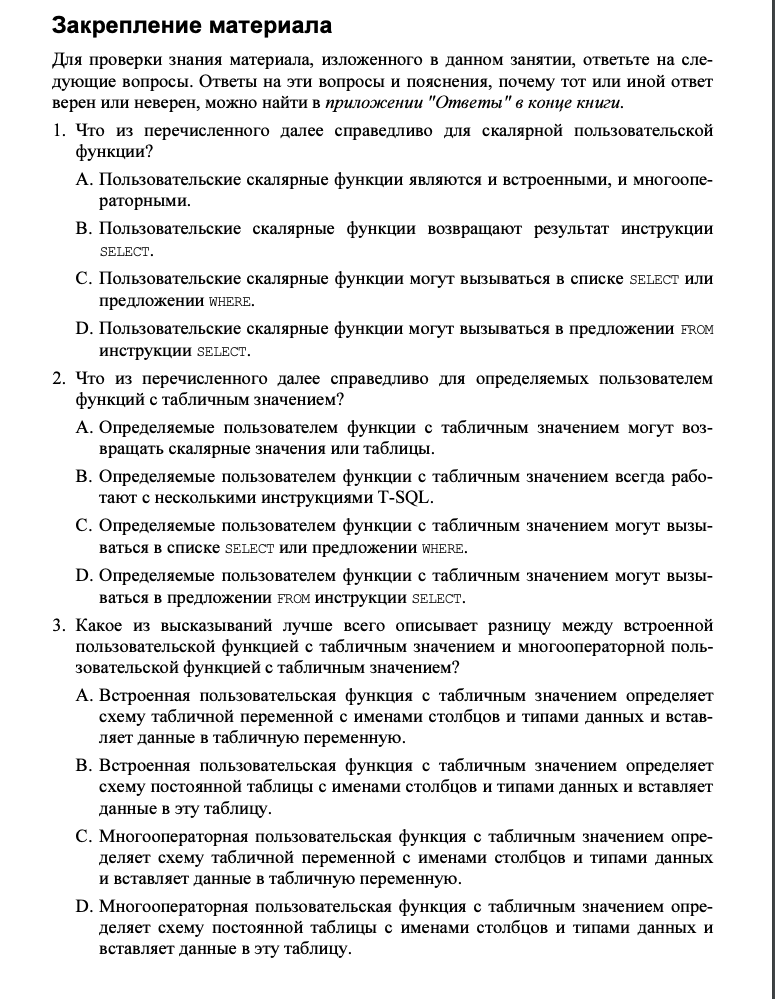
\includegraphics[width=0.7\textwidth]{img/zakrep32.png}
	\end{center}
	\captionsetup{justification=centering}
\end{figure}
\clearpage

\subsection*{Ответы}

\begin{figure}[h!]
	\begin{center}
		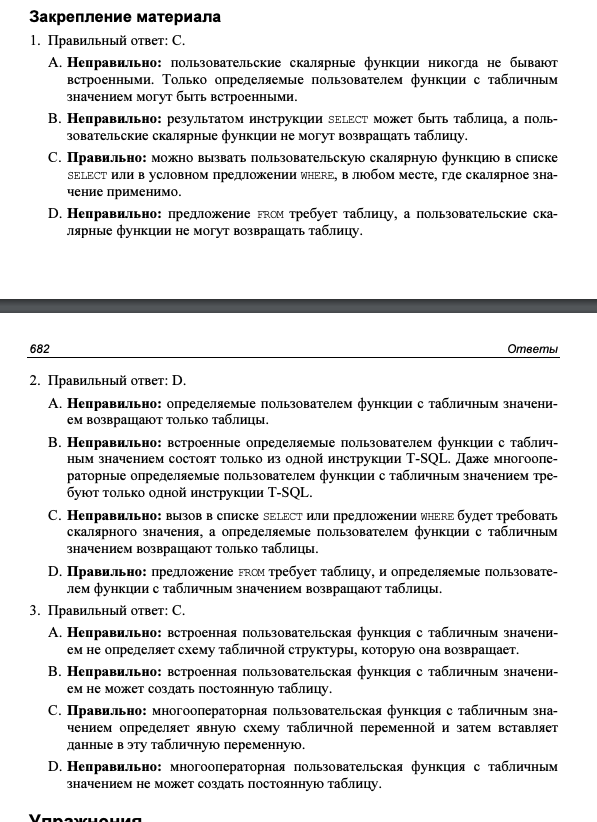
\includegraphics[width=0.9\textwidth]{img/ans32.png}
	\end{center}
	\captionsetup{justification=centering}
\end{figure}


\newpage
\subsection*{Упражнения}

\begin{figure}[h!]
	\begin{center}
		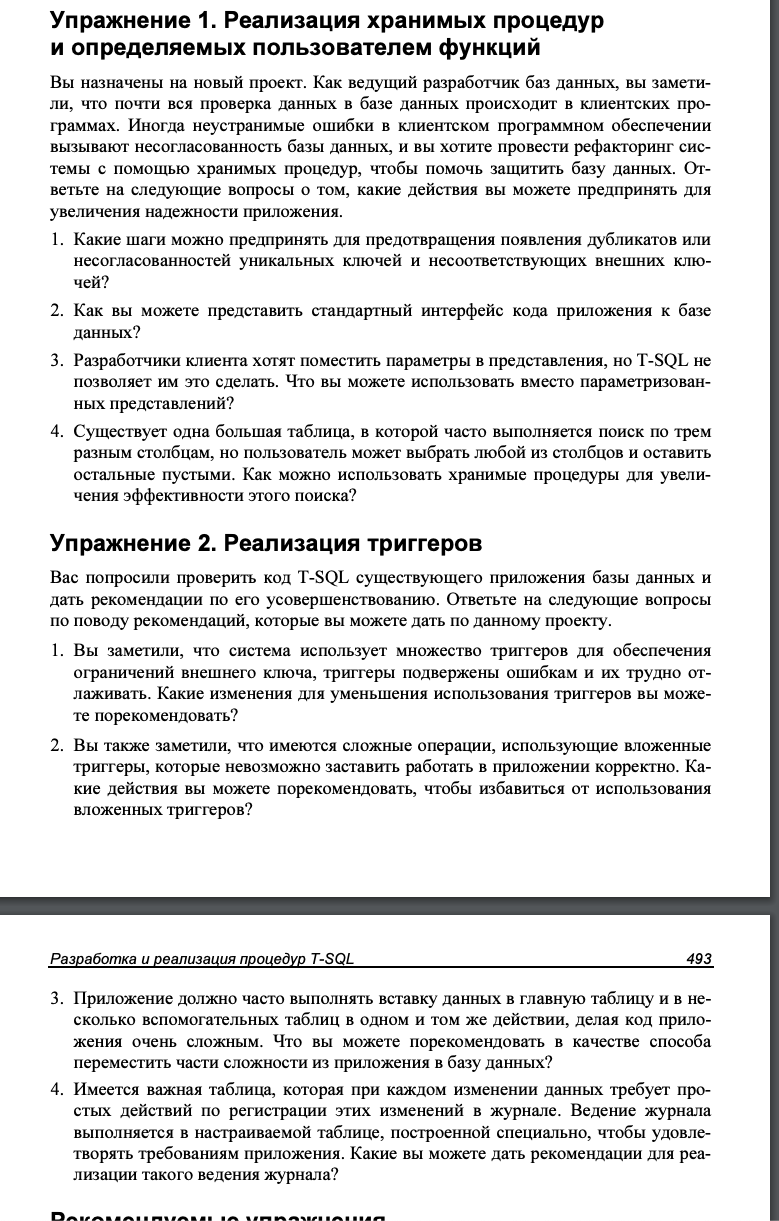
\includegraphics[width=0.9\textwidth]{img/ex30.png}
	\end{center}
	\captionsetup{justification=centering}
\end{figure}

\subsection*{Ответы}

\begin{figure}[h!]
	\begin{center}
		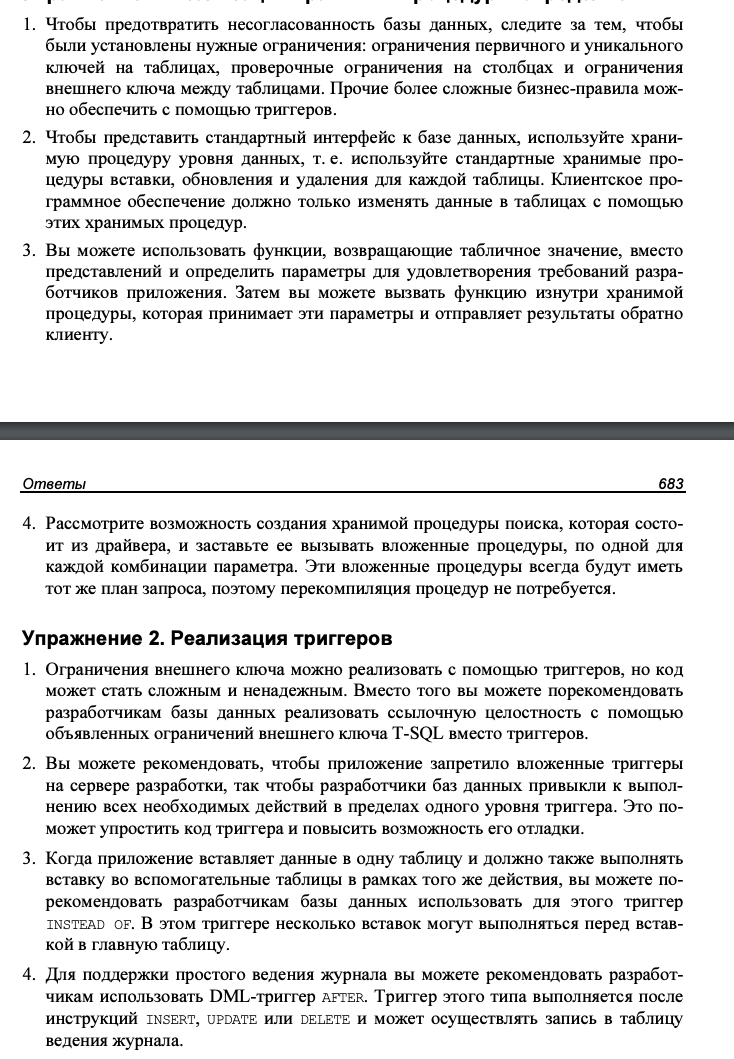
\includegraphics[width=0.9\textwidth]{img/eans30.png}
	\end{center}
	\captionsetup{justification=centering}
\end{figure}